\documentclass[11pt]{article}
\usepackage[margin=0.75in]{geometry}
\usepackage[T1]{fontenc}
\usepackage{helvet}
\renewcommand{\familydefault}{\sfdefault}
\usepackage{amsmath}
\usepackage{tikz}
\usepackage{array}
\usepackage{enumitem}
\pagestyle{empty}
\setlength{\parindent}{0pt}
\raggedright  % even word spacing, easier to read
\hyphenpenalty=10000 \exhyphenpenalty=10000  % never split a word across lines
\setlist[enumerate,2]{label=(\alph*),leftmargin=2em,itemsep=2.2em}

% Build the key with:  pdflatex -jobname=<name>_KEY "\def\iskey{}\input{<name>}"
\newif\ifkey
\ifdefined\iskey \keytrue \fi
\newcommand{\ans}[1]{\ifkey\leavevmode{\color{red!75!black}#1}\fi}

% ---------- helpers ----------
% dot plot: \dotplot{min}{max}{value/count,...}{axis label}
\newcommand{\dotplot}[4]{%
\begin{tikzpicture}[x=0.9cm,y=0.33cm]
  \draw[thick] (#1-0.5,0) -- (#2+0.5,0);
  \foreach \t in {#1,...,#2} {\draw (\t,0.25) -- (\t,-0.25) node[below] {\t};}
  \foreach \v/\c in {#3} {\ifnum\c>0 \foreach \k in {1,...,\c} {\fill (\v,\k*1.15) circle (0.16cm);}\fi}
  \node at ({(#1+#2)/2},-2.3) {#4};
\end{tikzpicture}}

% shape sketch: \shape{heights}{label}
\newcommand{\shapehist}[2]{%
  \foreach \h [count=\i from 0] in {#1} \draw[fill=gray!30] (\i,0) rectangle (\i+1,\h);
  \draw (-0.3,0) -- (12.3,0);
  \node[font=\bfseries] at (6,-2.6) {#2};}

% mean (triangle = balance point) and median (dashed line) markers
\newcommand{\meanmark}[1]{\fill (#1,0) -- ++(-0.3,-0.75) -- ++(0.6,0) -- cycle;}
\newcommand{\medmark}[2]{\draw[very thick,dashed] (#1,0) -- (#1,#2);}

\begin{document}

{\Large\bfseries Mean, Median, and Shape\ifkey\ \textcolor{red!75!black}{KEY}\fi}\hfill Name \underline{\hspace{2in}}

\vspace{0.8em}
\renewcommand{\arraystretch}{1.4}
\begin{tabular}{|>{\raggedright}p{3.25in}|>{\raggedright\arraybackslash}p{3.25in}|}
\hline
\textbf{Mean} (also called the \textbf{average}) &
\textbf{Median} (the \textbf{middle}) \\
1. Add all the values.\newline 2. Divide by how many values there are. &
1. Put the values in order.\newline 2. Find the middle value. \\
Data: \;2,\; 3,\; 8,\; 3,\; 4\newline
$2 + 3 + 8 + 3 + 4 = 20$ \quad\quad $20 \div 5 = 4$\newline
\textbf{Mean = 4}\newline
In symbols: \; $\bar{x} = \dfrac{\Sigma x}{n} = \dfrac{20}{5} = 4$ &
In order: \;2,\; 3,\; \fbox{3},\; 4,\; 8 \quad\quad \textbf{Median = 3}\newline
Even number of values? Two numbers are in the middle. Find the number halfway between them.\newline
2,\; \fbox{3},\; \fbox{5},\; 8 \quad\quad $(3 + 5) \div 2 = 4$ \quad \textbf{Median = 4} \\
\hline
\end{tabular}

\vspace{0.4em}
{\small $\Sigma$ is the Greek capital letter \textbf{sigma}. It means \textbf{add up}. \; $\Sigma x$ means add up all the values. \; $\bar{x}$ (``x-bar'') is the mean. \; $n$ is how many values.}

\vspace{0.8em}
\textbf{Shape changes the mean.} The \textbf{tail} is the long, low side of a graph.
The mean is \textbf{pulled toward the tail}. The median is not pulled much.

\vspace{0.6em}
\begin{center}
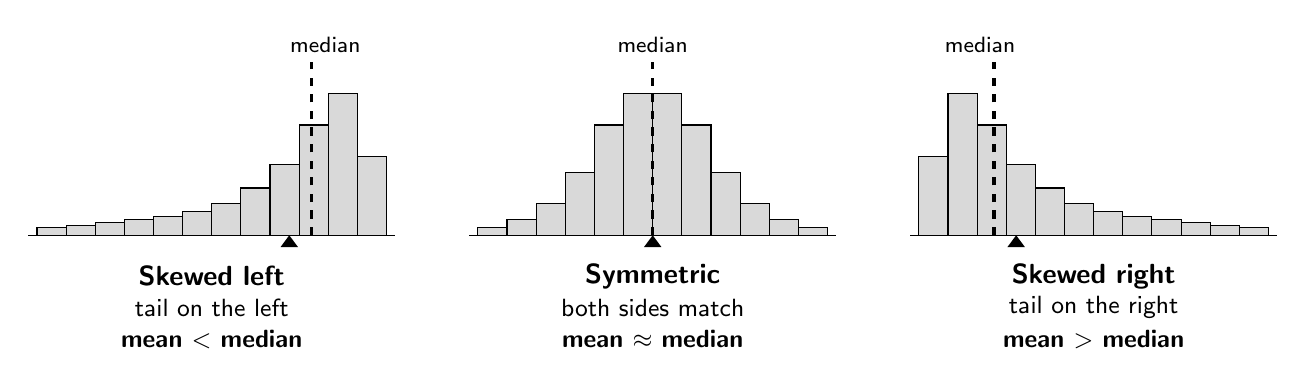
\begin{tikzpicture}[x=0.37cm,y=0.2cm]
\begin{scope}
  \shapehist{0.5,0.6,0.8,1,1.2,1.5,2,3,4.5,7,9,5}{Skewed left}
  \medmark{9.42}{11} \meanmark{8.66}
  \node[font=\footnotesize,anchor=south] at (9.9,11) {median};
  \node[font=\small] at (6,-4.6) {tail on the left};
  \node[font=\small] at (6,-6.6) {\textbf{mean $<$ median}};
\end{scope}
\begin{scope}[xshift=5.6cm]
  \shapehist{0.5,1,2,4,7,9,9,7,4,2,1,0.5}{Symmetric}
  \medmark{6}{11} \meanmark{6}
  \node[font=\footnotesize,anchor=south] at (6,11) {median};
  \node[font=\small] at (6,-4.6) {both sides match};
  \node[font=\small] at (6,-6.6) {\textbf{mean $\approx$ median}};
\end{scope}
\begin{scope}[xshift=11.2cm]
  \shapehist{5,9,7,4.5,3,2,1.5,1.2,1,0.8,0.6,0.5}{Skewed right}
  \medmark{2.58}{11} \meanmark{3.34}
  \node[font=\footnotesize,anchor=south] at (2.1,11) {median};
  \node[font=\small] at (6,-4.6) {tail on the right};
  \node[font=\small] at (6,-6.6) {\textbf{mean $>$ median}};
\end{scope}
\end{tikzpicture}

\vspace{0.3em}
\small\tikz\fill (0,0) -- (0.3,0) -- (0.15,0.22) -- cycle; = mean (the balance point) \qquad
\tikz\draw[very thick,dashed] (0,0) -- (0,0.3); = median\normalsize
\end{center}

\vspace{0.4em}
\textbf{Real example: US household income (2024).}
Most households earn a medium amount. A small number of households earn millions of dollars.
That makes a long tail on the right.

\begin{center}
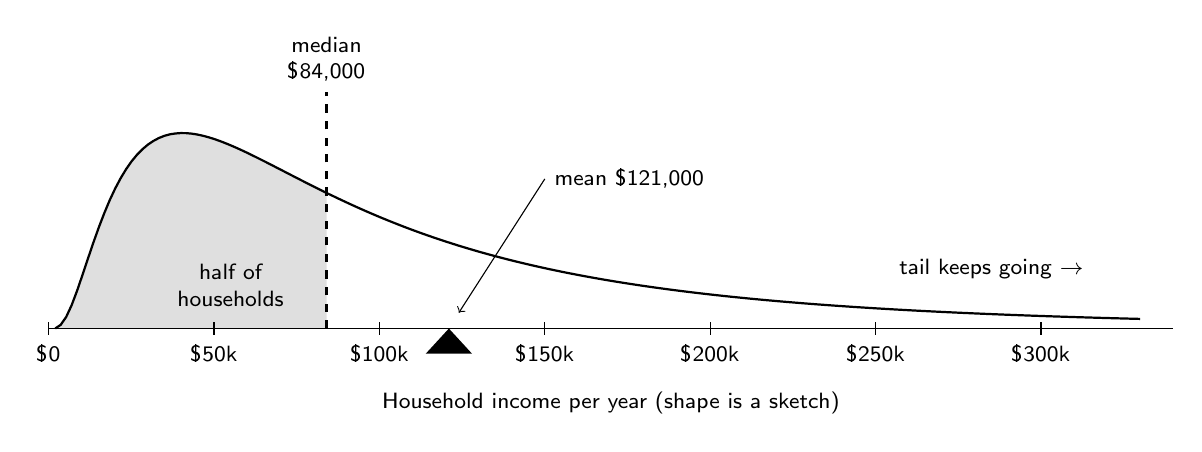
\begin{tikzpicture}[x=0.042cm,y=1cm]
  \def\mu{4.4308} \def\sg{0.855}
  \fill[gray!25] (2,0) -- plot[domain=2:84,samples=80] (\x,{310/(\x*\sg*2.5066)*exp(-((ln(\x)-\mu)^2)/(2*\sg*\sg))}) -- (84,0) -- cycle;
  \draw[thick] plot[domain=2:330,samples=200] (\x,{310/(\x*\sg*2.5066)*exp(-((ln(\x)-\mu)^2)/(2*\sg*\sg))});
  \draw (0,0) -- (340,0);
  \foreach \t/\l in {0/\$0,50/\$50k,100/\$100k,150/\$150k,200/\$200k,250/\$250k,300/\$300k}
    \draw (\t,0.08) -- (\t,-0.08) node[below,font=\footnotesize] {\l};
  \draw[very thick,dashed] (84,0) -- (84,3.0) node[above,font=\footnotesize,align=center] {median\\ \$84,000};
  \fill (121,0) -- ++(-7,-0.32) -- ++(14,0) -- cycle;
  \draw[->] (150,1.9) node[right,font=\footnotesize,align=left] {mean \$121,000} -- (124,0.2);
  \node[font=\footnotesize,align=center] at (55,0.55) {half of\\households};
  \node[font=\footnotesize] at (285,0.75) {tail keeps going $\rightarrow$};
  \node[font=\footnotesize] at (170,-0.95) {Household income per year (shape is a sketch)};
\end{tikzpicture}
\end{center}

The median is a better picture of a \textbf{typical} household. Most households earn \textbf{less than the mean}.

{\footnotesize Source: US Census Bureau, \textit{Income in the United States: 2024}. Median \$83,730. Mean about \$121,000.}

\vspace{0.3em}
Work with a partner. Compare answers when you finish each problem.

% ---------------- PROBLEMS ----------------
\newpage
\begin{enumerate}[leftmargin=1.5em,itemsep=1em]

\item A student recorded how many hours she slept each night for one week.
\begin{center}7,\; 8,\; 6,\; 9,\; 7,\; 5,\; 7\end{center}
\begin{enumerate}
  \item Find the mean. \ans{\quad $49 \div 7 = 7$ hours}
  \item Find the median. \ans{\quad 5, 6, 7, \fbox{7}, 7, 8, 9 \;$\rightarrow$\; 7 hours}
\end{enumerate}
\vspace{2.2em}

\item Six students timed their walk to the bus stop, in minutes.
\begin{center}15,\; 22,\; 18,\; 30,\; 19,\; 16\end{center}
\begin{enumerate}
  \item Find the mean. \ans{\quad $120 \div 6 = 20$ minutes}
  \item Find the median. \ans{\quad 15, 16, \fbox{18}, \fbox{19}, 22, 30 \;$\rightarrow$\; $(18 + 19) \div 2 = 18.5$ minutes. The 30 pulls the mean above the median.}
\end{enumerate}
\vspace{2.2em}

\item This dot plot shows how many books some students read this month.
\begin{center}\dotplot{0}{4}{0/1,1/3,2/5,3/4,4/2}{Books read this month}\end{center}
\begin{enumerate}
  \item How many students are in the data? \ans{\quad 15}
  \item Find the median. \ans{\quad The 8th value is 2 books.}
  \item Find the mean. \ans{\quad $(0 + 3 + 10 + 12 + 8) \div 15 = 33 \div 15 = 2.2$ books. Watch for: adding 0 to 4 instead of every dot.}
\end{enumerate}
\vspace{2.2em}

\newpage
\item A small company has 5 people. Here is what each person is paid in one year.
\begin{center}
\renewcommand{\arraystretch}{1.3}
\begin{tabular}{|l|r|} \hline
Worker A & \$30,000 \\ Worker B & \$32,000 \\ Worker C & \$35,000 \\ Worker D & \$38,000 \\ Owner & \$265,000 \\ \hline
\end{tabular}
\end{center}
\begin{enumerate}
  \item Find the mean pay. \ans{\quad $400{,}000 \div 5 = \$80{,}000$}
  \item Find the median pay. \ans{\quad \$35,000}
  \item The company puts this in a job ad: \textit{``Average pay at our company: \$80,000!''}
  Is this true? Is it fair to a person looking for a job? Explain.

  \ans{True, but not fair. 4 of the 5 people earn less than \$40,000. The owner's pay pulls the mean up. The median (\$35,000) is a better picture of a typical worker.}
  \item Leave out the owner. Find the mean pay of the 4 workers. How much did one person change the mean?

  \ans{$135{,}000 \div 4 = \$33{,}750$. One person moved the mean up by \$46,250.}
\end{enumerate}
\vspace{2.2em}

\newpage
\item Look at each histogram.

\begin{center}
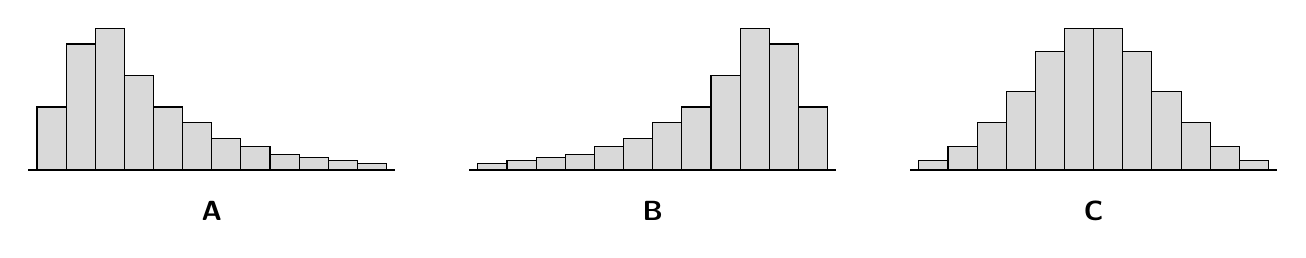
\begin{tikzpicture}[x=0.37cm,y=0.2cm]
\begin{scope}            \shapehist{4,8,9,6,4,3,2,1.5,1,0.8,0.6,0.4}{A} \end{scope}
\begin{scope}[xshift=5.6cm]  \shapehist{0.4,0.6,0.8,1,1.5,2,3,4,6,9,8,4}{B} \end{scope}
\begin{scope}[xshift=11.2cm] \shapehist{0.6,1.5,3,5,7.5,9,9,7.5,5,3,1.5,0.6}{C} \end{scope}
\end{tikzpicture}

\vspace{0.8em}
\renewcommand{\arraystretch}{2}
\begin{tabular}{|c|p{2in}|p{2.2in}|} \hline
Histogram & Shape & Mean $>$, $<$, or $\approx$ median? \\ \hline
A & \ans{skewed right} & \ans{mean $>$ median} \\ B & \ans{skewed left} & \ans{mean $<$ median} \\ C & \ans{symmetric} & \ans{mean $\approx$ median} \\ \hline
\end{tabular}
\end{center}
\vspace{1em}

\item Guess the shape of each data set: skewed left, symmetric, or skewed right. Explain.
\begin{enumerate}
  \item The price of every house sold in Columbia this year.

  \ans{Skewed right. Most houses are medium price. A few cost much more.}
  \item Scores on a very easy test. Most students score 90 to 100.

  \ans{Skewed left. Most scores are high. A few students score low.}
  \item The heights of all adult women in Missouri.

  \ans{Symmetric. Most heights are near the middle, with about as many tall as short.}
\end{enumerate}
\vspace{2.2em}

\item Look at the US household income graph on page 1.
\begin{enumerate}
  \item Why is the mean (\$121,000) bigger than the median (\$84,000)?

  \ans{Income is skewed right. A small number of very high incomes pull the mean toward the tail.}
  \item A news story says, \textit{``The average US household earns \$121,000.''}
  Is this true? Does it describe a typical household? Explain.

  \ans{It is true for the mean. It does not describe a typical household. Most households earn less. The median is a better picture.}
  \item Do more than half of households earn less than \$121,000? How do you know?

  \ans{Yes. Half of households earn less than \$84,000 (the median). Some more earn between \$84,000 and \$121,000.}
\end{enumerate}

\end{enumerate}

\end{document}
